In section \ref{section_frequency_distribution_tables}, frequency distribution tables were introduced to summarize the model validation results given a single constraint. However, the model-validation-result function might contain the validation result of multiple constraints. Hence, a way is needed to visualize the results in that case.

A natural extension of the last section is to create a frequency distribution table for each constraint using the same subset of indices $D_{idx}$, the same set of groups $G$, and the same set of possible validation results $V$. Given the constraints $c_j$ ($j \in [1,...,M]; M \in \mathbb{N}$), the frequency distribution tables $F_{G,V}^{c_j,D_{idx}}$ have the same dimensions and all sum up to $|D_{idx}|$. In most cases, the grouping will be defined without making use of the constraint validation results and, therefore, summing the validation results per group will be the same for all constraints. This motivates summarizing the model validation results in a histogram, having $M$ bars per group and each bar visualizes the distribution of the validation result for the given group.

\begin{Bsp}{Visualizing the Validation Results of Multiple Constraints Using a Histogram}{grouped_stacked_histogram}
This example extends example \ref{Bsp:class_per_constraint_samples_plot} by adding the constraint $C2$ expressing that males should not be vaccinated and the constraint $C3$ that females should be vaccinated in general. 
The following table gives the model-validation-result function $\Theta$ (short version of the table in example \ref{Bsp:evaluating_example_constraint} showing the validation results but for multiple constraints).

\captionsetup{type=htypei}
\begin{minipage}[t]{\linewidth}
    \vspace{1ex}
    \centering
    \begin{tabular}{cl|ccc}
        \toprule
        dataset indices $i$ & Person & $\Theta(C,i)$ & $\Theta(C2,i)$ & $\Theta(C3,i)$\\
        \midrule
        \midrule
        $1...3333$     & \uri{:Max} & -1 & 1 & -1\\
        $3334...4166$  & \uri{:Maria} & 0 & -1 & 0\\
        $4167...9166$  & \uri{:Eva} & -1 & -1 & 1\\\
        $9167...9999$  & \uri{:Laura} & -1 & -1 & 0\\
        \bottomrule
    \end{tabular}
    \captionof{table}{The model-validation-result function for the motivating example given the constraints $C$,$C2$ and $C3$}
    \label{fig:validation_results_summary_theta}
    \vspace{1ex}
\end{minipage}

As the frequency distribution tables are needed, $\mathcal{F}$ is executed as in in example \ref{Bsp:creating_frequency_distribution_tables} but for the constraint $C2$ and $C3$. The results of the executions are shown in the frequency distribution tables shown in Figure \ref{fig:frequency_distribution_table_second_motivating_constraint} and \ref{fig:frequency_distribution_table_third_motivating_constraint}.

Afterwards, all three frequency distribution tables (Figure \ref{fig:class_per_constraint_samples_table}, \ref{fig:frequency_distribution_table_second_motivating_constraint} and \ref{fig:frequency_distribution_table_third_motivating_constraint}) are visualized in Figure \ref{fig:class_per_constraints_samples_plot} using a histogram with a group of bars for each group (the predicted class) and each bar in the group for one of the constraints. Therefore, the validation results can be compared visually.

It turns out that all persons predicted to be vaccinated are females (valid according to $C3$). Further, approximately $\frac{2}{3}$ of the non-vaccinated persons are males (valid according to $C2$) and the rest of them are females (invalid according to $C$ and $C3$). 

As the motivating example, the constraint was a prediction constraint; the predictions, confirmed by the model validation results, can now be explained. In the example, there are 5,000 predictions valid according to $C3$ and 3,333 predictions valid according to $C2$. These predictions can now be explained with the conditions defined for $C2$ and $C3$, respectively. These predictions are correct because males should not be vaccinated, resp., females should be vaccinated.

   \captionsetup{type=htypei}
   \begin{minipage}[t]{\linewidth}
        \vspace{1ex}
        \centering
        \begin{tabular}{l|ccc}
            \toprule
             Groups & valid & invalid & not applicable \\
             \midrule
             vaccinated & 0 & 0 & 5000 \\
             not vaccinated & 3333 & 0 & 1666 \\
             \bottomrule
        \end{tabular}
        \captionof{figure}{Frequency distribution table $F_{\{\textrm{vaccinated},\textrm{not vaccinated}\},\{-1,0,1\}}$ for the constraint $C2$ using a grouping by the target class}
        \label{fig:frequency_distribution_table_second_motivating_constraint}
    \end{minipage}
   
   \captionsetup{type=htypei}  
   \begin{minipage}[t]{\linewidth}
        \vspace{1ex}
        \centering
        \begin{tabular}{l|ccc}
            \toprule
             Groups & valid & invalid & not applicable \\
             \midrule
             vaccinated & 5,000 & 0 & 0 \\
             not vaccinated & 0 & 1,666 & 3,333\\
             \bottomrule
        \end{tabular}
        \captionof{figure}{Frequency distribution table $F_{\{\textrm{vaccinated},\textrm{not vaccinated}\},\{-1,0,1\}}$ for the constraint $C3$ using a grouping by the target class}
        \label{fig:frequency_distribution_table_third_motivating_constraint}
    \end{minipage}
        \captionsetup{type=htypei}
        \begin{minipage}[t]{\linewidth}
            \vspace{1ex}
            \centering
            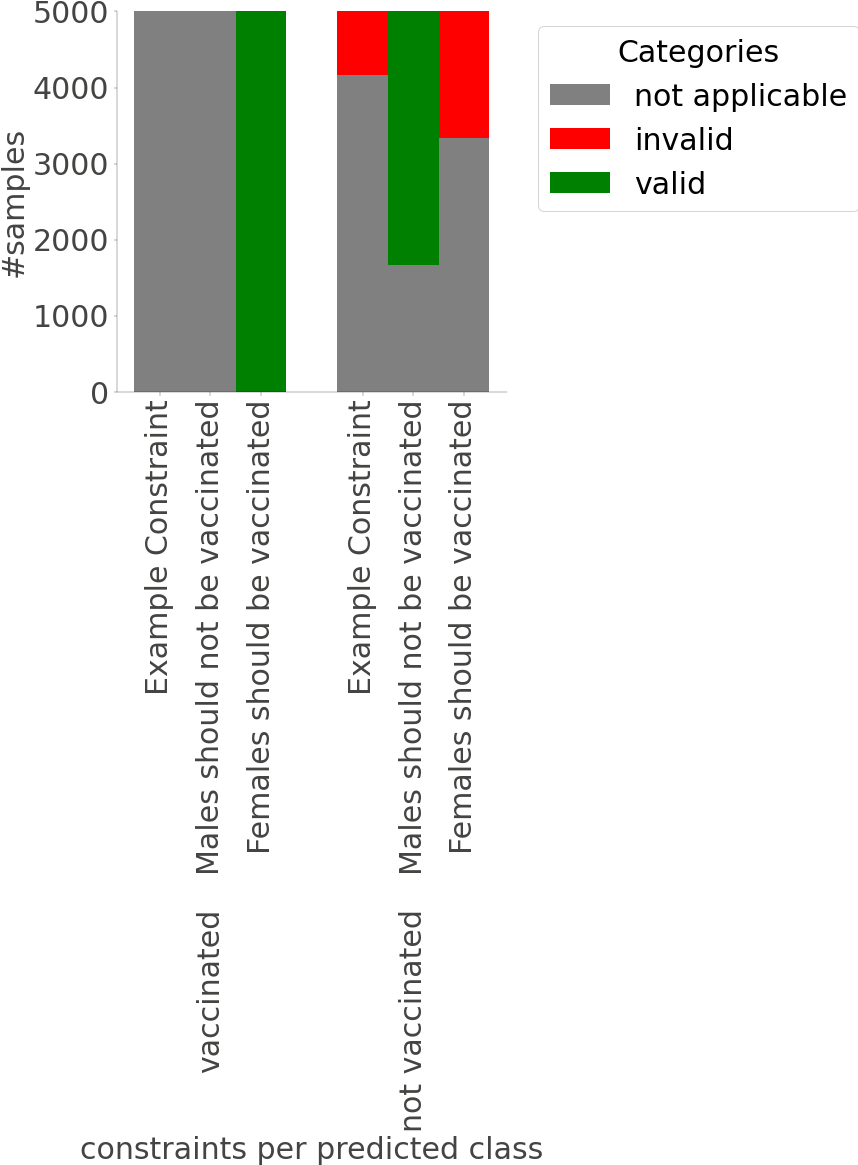
\includegraphics[scale=.25]{images/visualizations/example_constraints_per_predicted_class.png}    
            \captionof{figure}{Histogram of the frequency distribution tables in Figure \ref{fig:class_per_constraint_samples_table}, \ref{fig:frequency_distribution_table_second_motivating_constraint} and \ref{fig:frequency_distribution_table_third_motivating_constraint}}
            \label{fig:class_per_constraints_samples_plot}
        \end{minipage}
\end{Bsp}

This kind of visualization is great to compare the validation results per constraint. However, it stays unclear how the validation results of the different constraints are correlated, i.e., in general knowing how the validation results of the different constraints overlap. For example, one cannot say in general whether the instances invalidated by constraint $C$ are included in the ones invalidated by constraint $C3$ or whether there are predictions validated by $C2$ but invalidated by $C$ or $C3$. Another interesting question, in the case of the 3-valued logic, is whether all the predictions made by the model on the basis of the samples belonging to the subset of indices given are covered by at least one constraint. That is, there is a constraint $C$ for each index $i \in D_{idx}$ such that $\Theta(C,i) \neq -1$. To answer these kinds of questions, another function $COV$ is defined to create frequency distribution tables, which summarize the validation results of multiple constraints in a single 2-dimensional frequency distribution table.

\begin{Def}{A Function to Create Frequency Distribution Tables to Summarize the Model Validation Results of Multiple Constraints}{coverage}
Let $D$ be a dataset, $G$ a set of arbitrary group identifiers, $\mathcal{C}$ a tuple $(c_1, c_2, ...,c_M)$ of constraints with falling priority, $N$ the number of samples in $D$ and $\mathbf{\Gamma}$ the endless space of grouping function $\Gamma: G \to \mathcal{P}([1,...,N])$, then the function \[COV_{G,\mathcal{C}}: \mathcal{P}([1,...,N]) \times \mathbf{\Theta} \times \mathbf{\Gamma} \to \mathbb{N}^{|G| \times |\mathcal{C}| * |\{-1,0,1\}| }\]
 maps a subset of the indices $D_{idx}$ of $D$, a model validation result function $\Theta$ and a grouping function $\Gamma$ to a frequency distribution table:
 \[COV_{G,C}(D_{idx},\Theta, \Gamma) \mapsto \left(\left|c_{g,v}^{c_i,D_{idx}}\right|\right)_{\substack{g \in G\\ (v,c_i) \in (\{-1,0,1\} \times \mathcal{C}) }}\]
 where 
 \begin{align*}
     c_{g,0}^{c_i,D_{idx}} & = f_{g,0}^{c_i,D_{idx}} \setminus \left(\bigcup_{j < i} f_{g,0}^{c_j,D_{idx}}\right)\\
     c_{g,1}^{c_i,D_{idx}} & = f_{g,1}^{c_i,D_{idx}} \setminus \left(\bigcup_{j < i} f_{g,1}^{c_j,D_{idx}} \cup \bigcup_{i} f_{g,0}^{c_j,D_{idx}}\right)\\
     c_{g,-1}^{c_i,D_{idx}} & = f_{g,-1}^{c_i,D_{idx}} \setminus \left(\bigcup_{j < i} f_{g,-1}^{c_j,D_{idx}} \cup \bigcup_{i} f_{g,0}^{c_j,D_{idx}} \cup \bigcup_{i} f_{g,1}^{c_j,D_{idx}}\right)\\
 \end{align*}
 and $f_{g,v}^{c_i,D_{idx}}$ is defined as in definition \ref{Def:frequency_distribution_creation_function}.
\end{Def}

As in definition \ref{Def:frequency_distribution_creation_function}, the sum of the entries is $|D_{idx}|$ per table. However, definition \ref{Def:coverage} summarizes the validation results of $|\mathcal{C}| * |D_{idx}|$ validation results by only counting the ones with the highest priority. Therefore, a tuple of constraints $\mathcal{C}$ with falling priority is needed and, furthermore, it is assumed that an invalided prediction has a higher importance than a valid prediction, which in turn is more important than a non-applicable one. Given these priorities, it is possible to count exactly one validation result per sample. 

When using the 3-valued logic, the resulting frequency distribution table shows the coverage of the validation results over the subset of samples (i.e., the number of validation results are not \emph{not applicable}). Due to this, the summarization method from definition \ref{Def:coverage} will be referred to by \emph{coverage}.

\begin{Bsp}{Applying Definition \ref{Def:coverage} to Example \ref{Bsp:grouped_stacked_histogram}}{coverage_example}
In this example, the constraint validation results from \ref{Bsp:grouped_stacked_histogram} are reused and definition \ref{Def:coverage} is applied as follows.
First, the inputs are determined:
\begin{align*}
    G = & \{\text{vaccinated}, \text{not vaccinated}\} \\
    \mathcal{C} = & \text{tuple}(\{C,C1,C2\}) =: (c_1,c_2,c_3) \\
    N = 9999 = & |D| \\
    D_{full} = & [1,...,N] \\
\end{align*}
where $D$ is the usual motivating example dataset and $\Gamma_{\textrm{ground truth class}}$ the grouping function from example \ref{Bsp:creating_frequency_distribution_tables}.
To execute \[COV_{G,\mathcal{C}}(D_{full},\Theta,\Gamma_{\textrm{ground truth class}})\] first, the sets $f_{g,v}^{c_i,D_{full}}$ need to be estimated for all $g \in G$, $v \in \{-1,0,1\}$ and $i \in \{1,2,3\}$. This is done in Figure \ref{fig:frequency_distribution_entries_all_constraints} using the ground truth values from Figure \ref{fig:motivating_dataset}.

\captionsetup{type=htypei}
\begin{minipage}[t]{\linewidth}
    \vspace{1ex}
    \centering
    \begin{tabular}{l|ll}
        \toprule
        $(v,c_i)$ & $f_{\text{vaccinated},v}^{c_i,D_{full}}$ & $f_{\text{not vaccinated},v}^{c_i,D_{full}}$\\
        \midrule
        \midrule
        $(0,c_1)$ & $\emptyset$ & $[3334,...,4166]$ \\
        $(0,c_2)$ & $\emptyset$ & $\emptyset$\\
        $(0,c_3)$ & $\emptyset$ & $[3334,...,4166] \cup [9167,...,9999]$\\
        $(1,c_1)$ & $\emptyset$ & $\emptyset$\\
        $(1,c_2)$ & $\emptyset$ & $[1,...,3333]$\\
        $(1,c_3)$ & $[4167,...,9166]$ & $\emptyset$\\
        $(-1,c_1)$ & $[4167,...,9166]$ & $[1,...,3333] \cup [9167,...,9999]$ \\
        $(-1,c_2)$ & $[4167,...,9166]$ & $[3334,...,4166] \cup [9167,...,9999]$ \\
        $(-1,c_3)$ & $\emptyset$ & $[1,...,3333]$ \\
        \bottomrule
    \end{tabular}
    \captionof{figure}{Table showing the $f_{g,v}^{c_i,D_{full}}$}
    \label{fig:frequency_distribution_entries_all_constraints}
    \vspace{1ex}
\end{minipage}
Building on the sets $f_{g,v}^{c_i,D_{full}}$, the sets $c_{g,v}^{c_i,D_{idx}}$ can be estimated as in Figure \ref{fig:coverage_frequency_distribution_entries_all_constraints}.

\captionsetup{type=htypei}
\begin{minipage}[t]{\linewidth}
    \vspace{1ex}
    \centering
    \begin{tabular}{l|ll}
        \toprule
        $(v,c_i)$ & $c_{\text{vaccinated},v}^{c_i,D_{full}}$ & $c_{\text{not vaccinated},v}^{c_i,D_{full}}$\\
        \midrule
        \midrule
        $(0,c_1)$ & $\emptyset$ & $[3334,...,4166]$ \\
        $(0,c_2)$ & $\emptyset$ & $\emptyset$\\
        $(0,c_3)$ & $\emptyset$ & $[9167,...,9999]$\\
        $(1,c_1)$ & $\emptyset$ & $\emptyset$\\
        $(1,c_2)$ & $\emptyset$ & $[1,...,3333]$\\
        $(1,c_3)$ & $[4167,...,9166]$ & $\emptyset$\\
        $(-1,c_1)$ & $\emptyset$ & $\emptyset$ \\
        $(-1,c_2)$ & $\emptyset$ & $\emptyset$ \\
        $(-1,c_3)$ & $\emptyset$ & $\emptyset$ \\
        \bottomrule
    \end{tabular}
    \captionof{figure}{Table showing the $c_{g,v}^{c_i,D_{full}}$}
    \label{fig:coverage_frequency_distribution_entries_all_constraints}
    \vspace{1ex}
\end{minipage}

Finally, taking the cardinality of the sets give the frequency distribution table.
   \captionsetup{type=htypei}
   \begin{minipage}[t]{\linewidth}
        \vspace{1ex}
        \centering
        \begin{tabular}{l|cccc}
            \toprule
             Groups & $(c_1,0)$ & $(c_2,0)$ & $(c_2,1)$ & $(c_3,1)$ \\
             \midrule
             vaccinated & 0 & 0 & 5000 & 0 \\
             not vaccinated & 833 & 833 & 0 & 3333\\
             \bottomrule
        \end{tabular}
        \captionof{figure}{Frequency distribution table showing the coverage results for the constraints $c_1,c_2,c_3$ using a grouping by the ground truth class}
        \label{fig:frequency_distribution_table_coverage}
        \vspace{1ex}
    \end{minipage}

    The frequency distribution table can now be visualized as usual. This is done in Figure \ref{coverage_dataset} using the grouping by the ground truth class on the left side and without a grouping on the right side. In comparison to Figure \ref{fig:class_per_constraints_samples_plot}, it becomes clear that all the predictions made by the model are covered by at least one constraint. In the case of predictions not covered by any constraint, these will always fall in the $(-1,c_1)$ category, which will be called \emph{not covered} in future visualizations.
    
    Further, the plot allows making statements about the overlapping of validation results. A prediction marked as valid is not invalidated by any other constraint. A lesser important constraint validation result can only be overlapped by a more important one, given that the validation result is the same. Therefore, in the example approximately $83\%$ of the samples in the dataset are predicted according to the constraints and approximately $8\%$ is invalidated by the example constraint and another $8\%$ is invalidated by the second constraint, but not by the example constraint.
   
   \captionsetup{type=htypei}
   \begin{minipage}[t]{\linewidth}
    \vspace{1ex}
    \centering
        \begin{minipage}[t]{0.25\linewidth}
            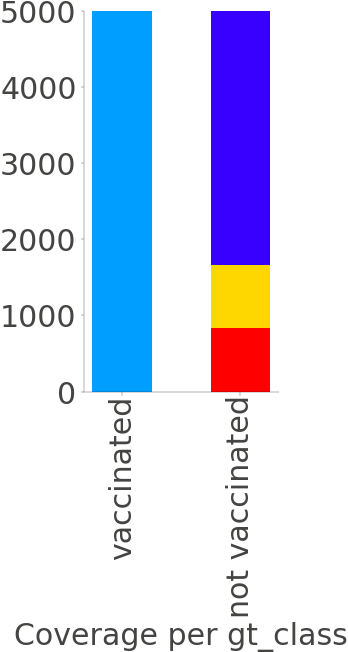
\includegraphics[scale=.25]{images/visualizations/coverage_constraints_gt_class.png}
        \end{minipage}
        \hspace{1ex}
        \begin{minipage}[t]{0.7\linewidth}
            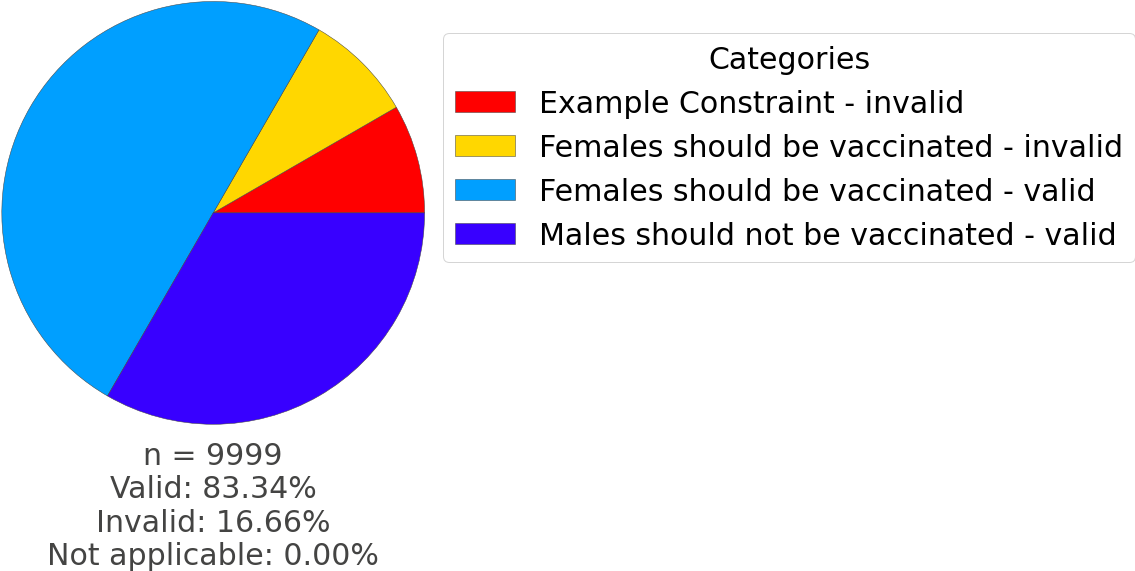
\includegraphics[scale=.25]{images/visualizations/coverage_constraints_pie.png}
        \end{minipage}
    \captionof{figure}{Validation Results of multiple constraints summarized by coverage. Left side shows the results grouped by the ground truth class and the right side shows the results without a grouping}
    \label{coverage_dataset}
    \vspace{1ex}
    \end{minipage}
\end{Bsp}